\chapter{Foundations}\label{ch:foundation}

\section{Game environment}\label{sec:game_environment}
To support our research activity, we have designed and implemented a new \gls{pirg}. 
%ANDY to each paragraph a motivation for the choice should be reported, possibly referring to something already mentioned in the section about the state of art, about PIRG design. The aim is not only to describe the playground, but to support somehow the decisions with some methodological finding.
\\
The playground consists of a rectangular area of 4m$\times$4m where, on each corner, tubes (henceforth called ``towers'') were placed. Each tower is equipped with a button (which sits on the tower's cap) and four~\gls{led}s that can be progressively turned on, one by one.  Each~\gls{led} requires the button to be pressed for 2.5 seconds, meaning that the tower takes about 10 seconds of button push in order to light up all of the four~\gls{led}s.

The~\gls{led}s are supposed to display the progress of the human player in capturing a specific tower. For a given tower, after turning on all~\gls{led}s, it is said that the player has captured it; Figure~\ref{tubes} presents the towers that were used in the game. When a tower is secured, the robot cannot aim at it anymore.
Button pressing time is cumulative and can be distributed on different moments -- this means that the player will not lose his progress if he stops pressing the button before the tower is completely captured. 

In order to win, the human player must be able to secure all the existing towers without letting a single one be knocked down by the robot. If, at anytime, a tower falls (because of the robot or the player) the game ends and the human player is losing. 

The robot is able to move across the entire playground just as the human player and it is only constrained by the fact that an already captured tower, or one whose button is currently being pressed by the player, cannot be teared down. The player can also block the robot path by staying in front of it, causing the later to likely change target tower. Notice that, while the player is trying to capture a given tower, the robot can try to tear down any other one.

%ANDY This would go in the robot description -> By relying on the lasers scans the robot can perceive its environment, locate itself and the human player during the game, being able to perform obstacle avoidance when appropriated.

This game is designed so that the robot, given its agility and maximum speed (1.4 m/sec) could always win, but it should show the appropriate and believable behavior to keep the player engaged and interested. %ANDY Here is one of the places were the smartness of game design has to be put in evidence.

%\begin{figure}[H]
%	\centering
%	\begin{subfigure}[b]{0.4\textwidth}
%		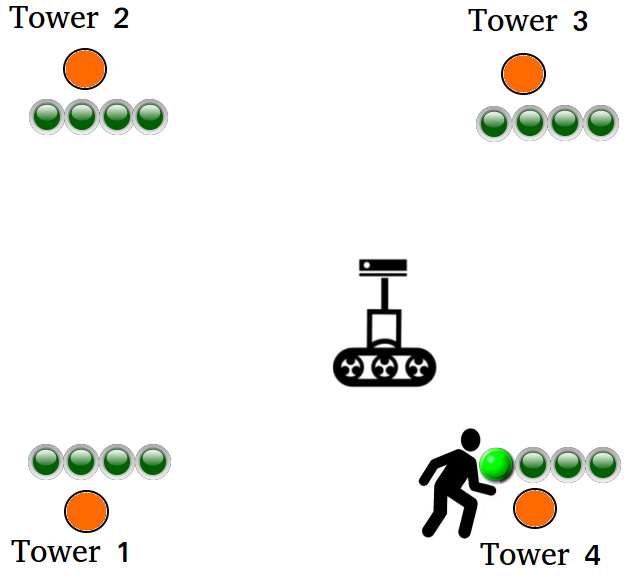
\includegraphics[width=5cm]{Chapter4/Figs/situation1}
%		\caption{Initial situation: player is capturing Tower-4}
%		\label{situation1} 
%	\end{subfigure}
%	\begin{subfigure}[b]{0.4\textwidth}
%		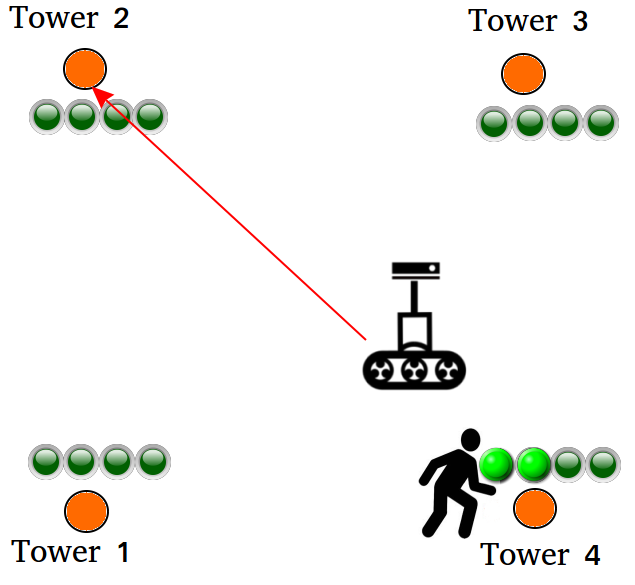
\includegraphics[width=5cm]{Chapter4/Figs/situation2}
%		\caption{Robot start moving in order to attack and tear down Tower-2}
%		\label{situation2}
%	\end{subfigure}
%	\begin{subfigure}[b]{0.4\textwidth}
%		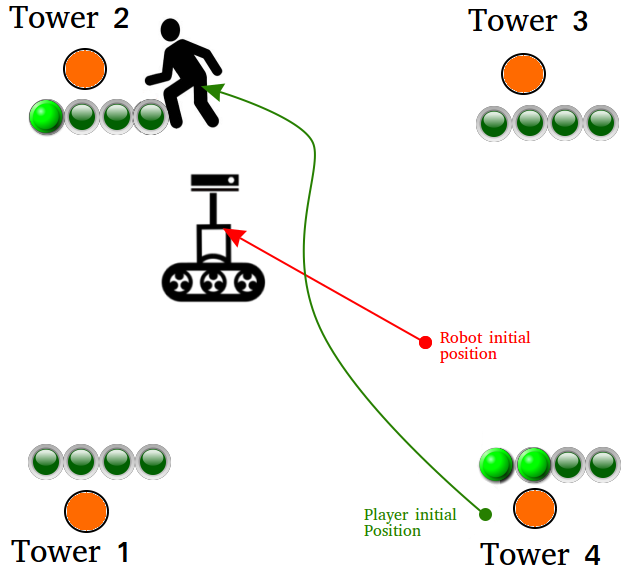
\includegraphics[width=5cm]{Chapter4/Figs/situation3}
%		\caption{Human player defends and start capturing Tower-2} 
%		\label{situation3}
%	\end{subfigure}
%	\begin{subfigure}[b]{0.4\textwidth}\centering
%		\includegraphics[width=3cm]{Chapter4/Figs/tubes}
%		\caption{Real towers that are used during the game}
%		\label{tubes} 
%	\end{subfigure}
%	\rule{35em}{0.5pt}
%	\caption{Schematic representation of the game:}
%	\label{overallgame}
%\end{figure}
%\begin{itemize}
%	\item figure~\ref{situation1}: The player is capturing the tower, when all the four LEDs are lit on the tower.
%	\item figure~\ref{situation2}: The robot attacks a Tower, it cannot try to tear down the tower that is currently being captured by the player.
%	\item figure~\ref{situation3}: The player stops the action of the robot by blocking its trajectory and defending the attacked tower. \textit{Please notice} how the progress on Tower-4 is not lost even if the player dismiss capturing it.
%\end{itemize}

During the game, the robot must be able to track the movements of the human player while navigating the path through the various target towers mainly to collect information on the activity level of its opponent (chapter~\ref{chapter4}). Details about the robot platform is given in section~\ref{sec:roboplat}.

%\begin{figure}[H]
%	\centering
%	\includegraphics[width=10cm]{Chapter5/Figs/im1}
%	\rule{35em}{0.5pt}
%	\caption{Moving robot tracking the movements of a human.}
%	\label{trackingconcept1} 
%\end{figure}

%To obtain the data from the human player that are needed to perform the tracking we used the Microsoft Kinect presented in~\ref{kinectsec} and a computer vision algorithm for blob detection previously integrated in the ROS environment using OpenCV libraries.

\section{Towers}\label{sec:towers}
Each tower is powered individually, being capable of transmitting its status to the robot at a constant rate. The circuit uses the NodeMCU V3 ESP8266 ESP-12E WiFi module\footnote{\url{https://einstronic.com/wp-content/uploads/2017/06/NodeMCU-ESP8266-ESP-12E-Catalogue.pdf} accessed on December 17th, 2018.} whose connection is done via a private network. The communication between towers and the robot is supported through TCP protocol using the rosserial\_server\footnote{\url{http://wiki.ros.org/rosserial_server} accessed on December 17th, 2018.} package. Figure~\ref{fig:tower_board} presents the board together with its pinout. 

\begin{figure}[thpb]
  \centering
  \begin{subfigure}[b]{\textwidth}
  	\centering
      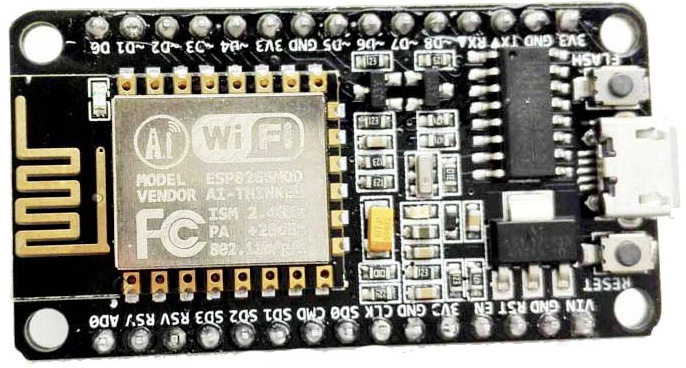
\includegraphics[width=5cm]{images/03-foundation/node_mcu}
	\caption{}
  \end{subfigure}
   \qquad 
  \begin{subfigure}[b]{\textwidth}
  \centering
      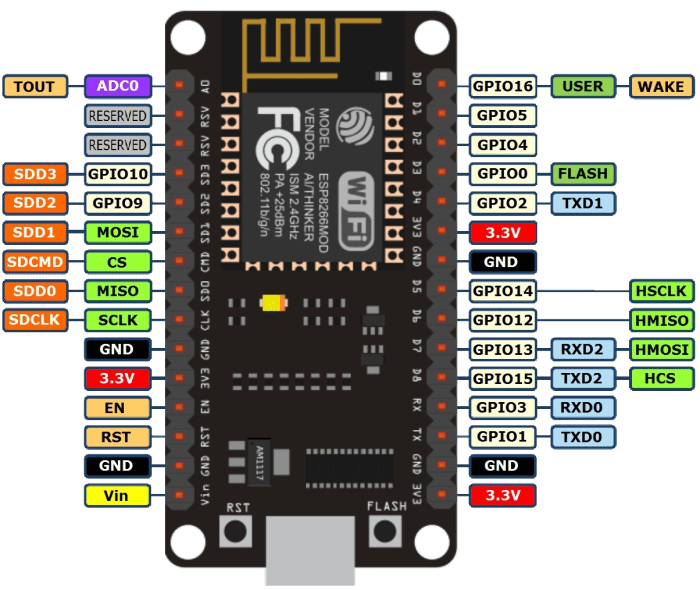
\includegraphics[width=5cm]{images/03-foundation/node_mcu_pinout}
	\caption{}
  \end{subfigure}
  \caption{a) The NodeMCU V3 ESP8266 ESP-12E WiFi module used for data transmission. b) module pinout.}
  \label{fig:tower_board}
\end{figure}

A $7.4$V LiPo battery is used on each tower as can been seen on figure~\ref{fig:tower_caps}. The nominal voltage for the boards is $5$V, which is supplied through a voltage regulator. %An angle switch %ANDY What is this? A tilt sensor?
A tilt sensor allows the detection of fallen towers. A schematic of the circuit developed to detect such event is provided in figure~\ref{fig:tilt_circuit}.

\begin{figure}[H]
  \centering
  \begin{subfigure}[t]{0.33\textwidth}
  	\centering
    \includegraphics[width=3cm, height=5cm]{images/03-foundation/cap1}
	\caption{}
  \end{subfigure}
  ~ 
  \begin{subfigure}[t]{0.33\textwidth}
  	\centering
    \includegraphics[width=3cm, height=5cm]{images/03-foundation/cap2}
	\caption{}
  \end{subfigure}
  ~
   \begin{subfigure}[b]{0.33\textwidth}
	  \centering
      \includegraphics[width=3cm,  height=5cm]{images/04-activity/tubes.jpg}
      \caption{}
    \end{subfigure}
  \caption{a) Tower cap containing the button and \gls{led}s; b) Tower cap circuit; c) The four towers used in the game (height 110cm).}
  \label{fig:tower_caps}
\end{figure}


\begin{figure}[H]
	\centering
		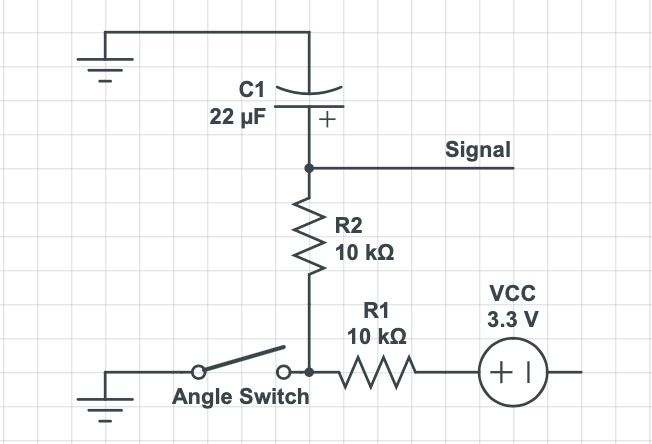
\includegraphics[width=0.5\textwidth, height=5cm]{images/03-foundation/tilt_sensor_circuit}
	\caption{The circuit for detecting when a tower has fallen. An angle switch detects the inclination and the low-pass filter smooths out noise from vibrations such as those caused by the player touching the tower. The signal wire is attached to a pin on the NodeMCU V3 ESP8266 ESP-12E WiFi Module, which allows communication with the robot's onboard computer.}
    \label{fig:tilt_circuit} 
\end{figure}

\section{The robotic platform}\label{sec:roboplat} 
We have designed an holonomic robot as experimental platform. This robot, called Triskar, is free to move in any direction at a speed comparable to that of people in indoor environments (up to 1.4~m/sec).The base consists of a metallic, triangular-shaped structure where motors, batteries, computer and necessary electronics are embedded. Triskar has simultaneously and independently controlled rotational and translational motion capabilities all thanks to three omni-directional wheels actuated by a motor each. The movement on flat floor abilities are similar to those of a good human player, as well as its projection of the ground plane, thus making Triskar a good base for PIRGs, in particular the one that we have designed. 

During the research progress, we have designed several versions of Triskar, where the first two had an overall height of 85~cm, so comparable to that of kid players, but also acceptable for adult players. The first three versions were adopting a Kinect\textsuperscript{\textregistered} sensor on top aimed at player tracking. Given the need to improve robustness, we have redefined the base by making structural changes to limit vibrations and improve stability of the sensors, which increased the overall high to 1 meter (3rd version). We also added new sensors such as planar laser scans needed to obtain reliable obstacle avoidance (3rd and 4th version). Figure~\ref{fig:evolution} depicts our prototype evolution. Finally, on the fourth version we dropped the 3-D camera, deemed to be too much unreliable for player detection, and devised for this goal algorithms based on laser scans only. We kept the height in the same range as before, for the mentioned reasons, although it was no longer needed to hold Kinect\textsuperscript{\textregistered}. To justify the height and give a character to the robot, we added eyes and hair on top, which were appreciated by players.

\begin{figure}[H]
      \centering
      \begin{subfigure}[b]{0.3\textwidth}
      	\centering
	    \framebox{\parbox{3cm}{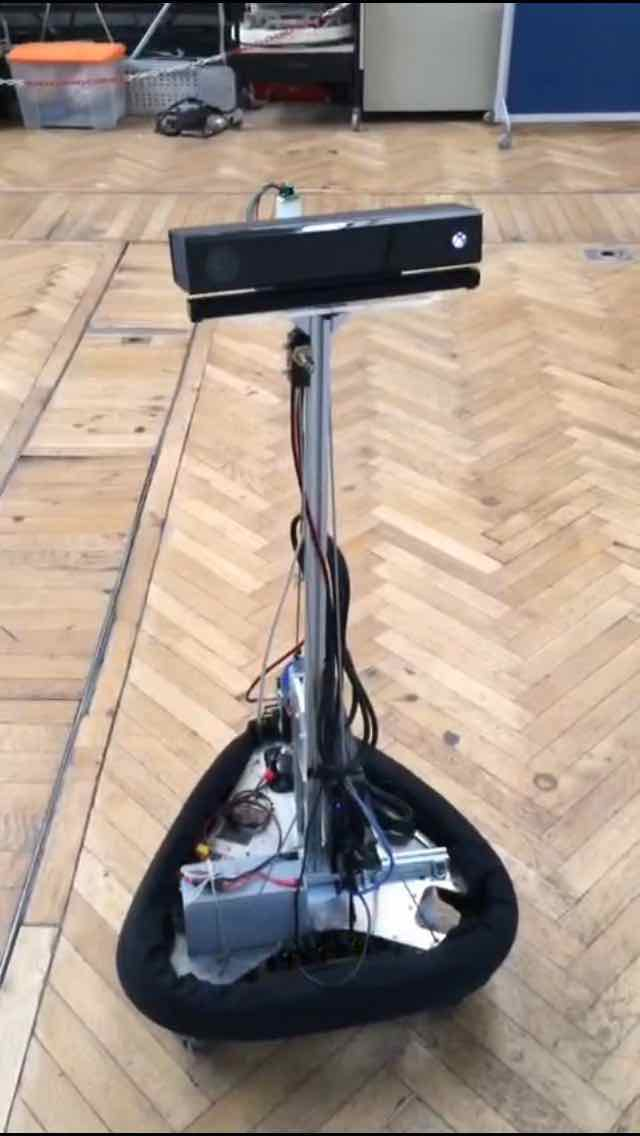
\includegraphics[width=3cm%, height=5.4cm
	    ]{images/03-foundation/base1}}}
	  	\caption{}
      \end{subfigure}
	 ~
	 \begin{subfigure}[b]{0.3\textwidth}
	 	\centering
		\framebox{\parbox{3cm}{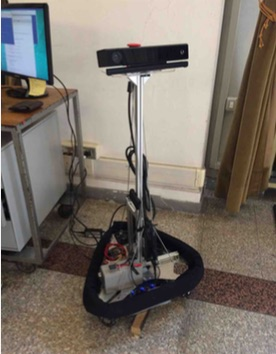
\includegraphics[width=3cm%, height=5.4cm
		]{images/03-foundation/base2}}}  
		\caption{}   
      \end{subfigure}
	 ~
	  \begin{subfigure}[b]{0.3\textwidth}
		\centering
	  	\framebox{\parbox{3cm}{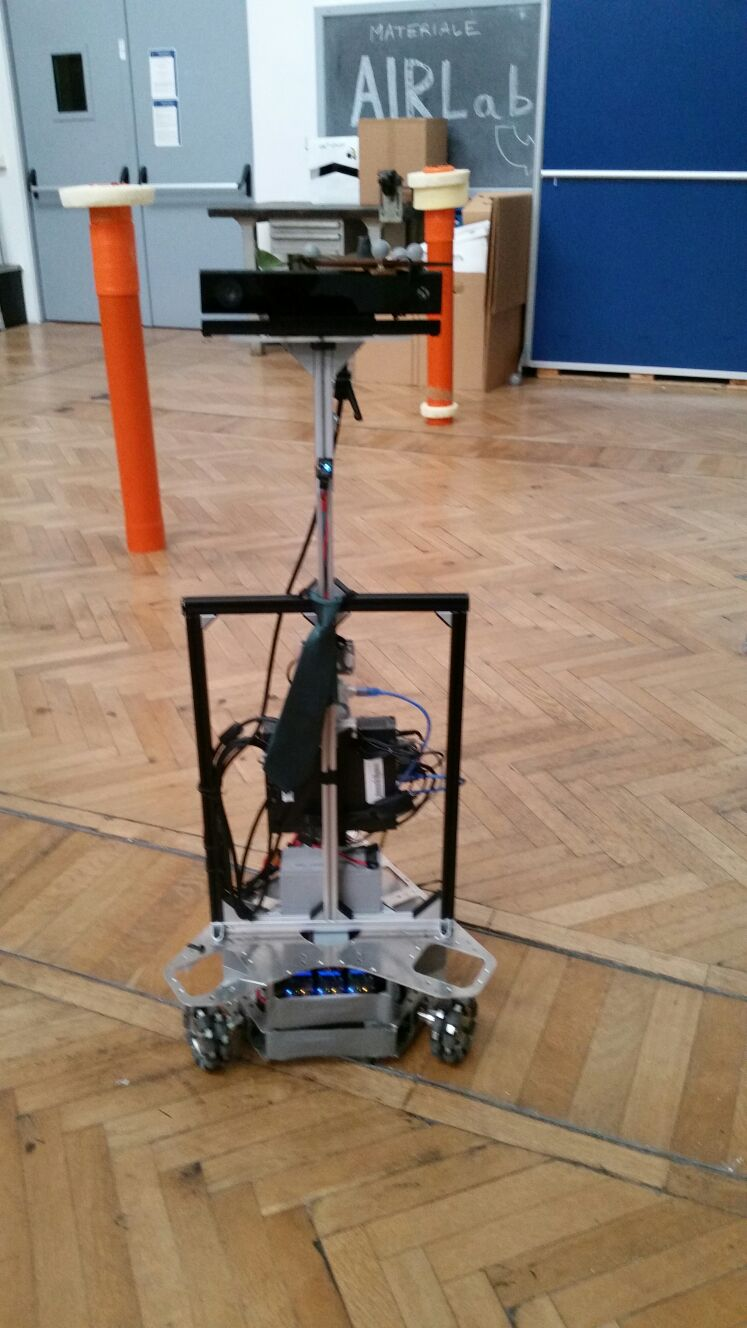
\includegraphics[width=3cm%,height=5.4cm
	  	]{images/03-foundation/mobilerobot.jpeg}}}
	  	\caption{}\label{robot}
      \end{subfigure}
      ~
      \begin{subfigure}[b]{0.3\textwidth}
      	\centering
      	\framebox{\parbox{3cm}{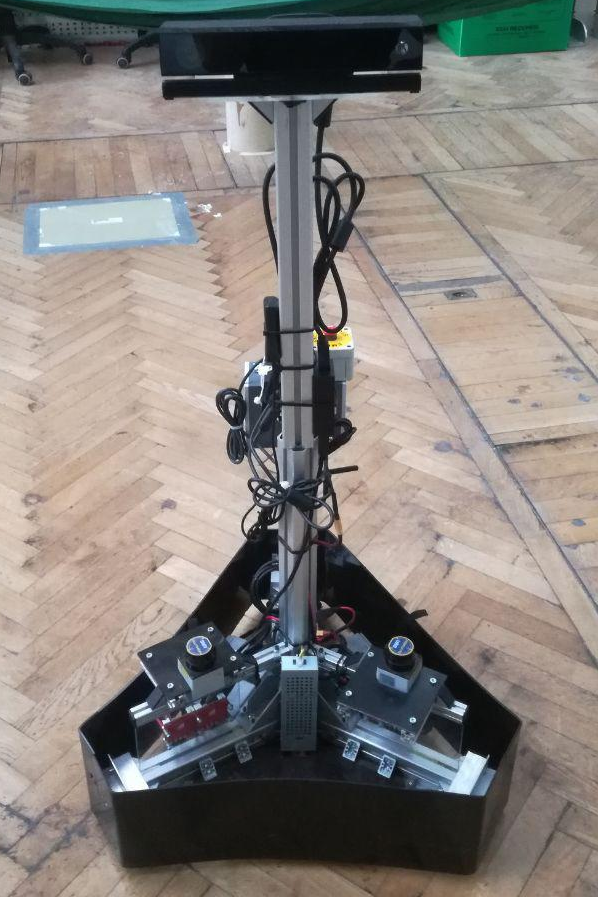
\includegraphics[width=3cm%,height=5.4cm
      	]{images/03-foundation/newmobilerobot.png}}}\label{newrobot}
      	\caption{}
      \end{subfigure}
      ~
      \begin{subfigure}[b]{0.3\textwidth}
	      \centering
	      \framebox{\parbox{3cm}{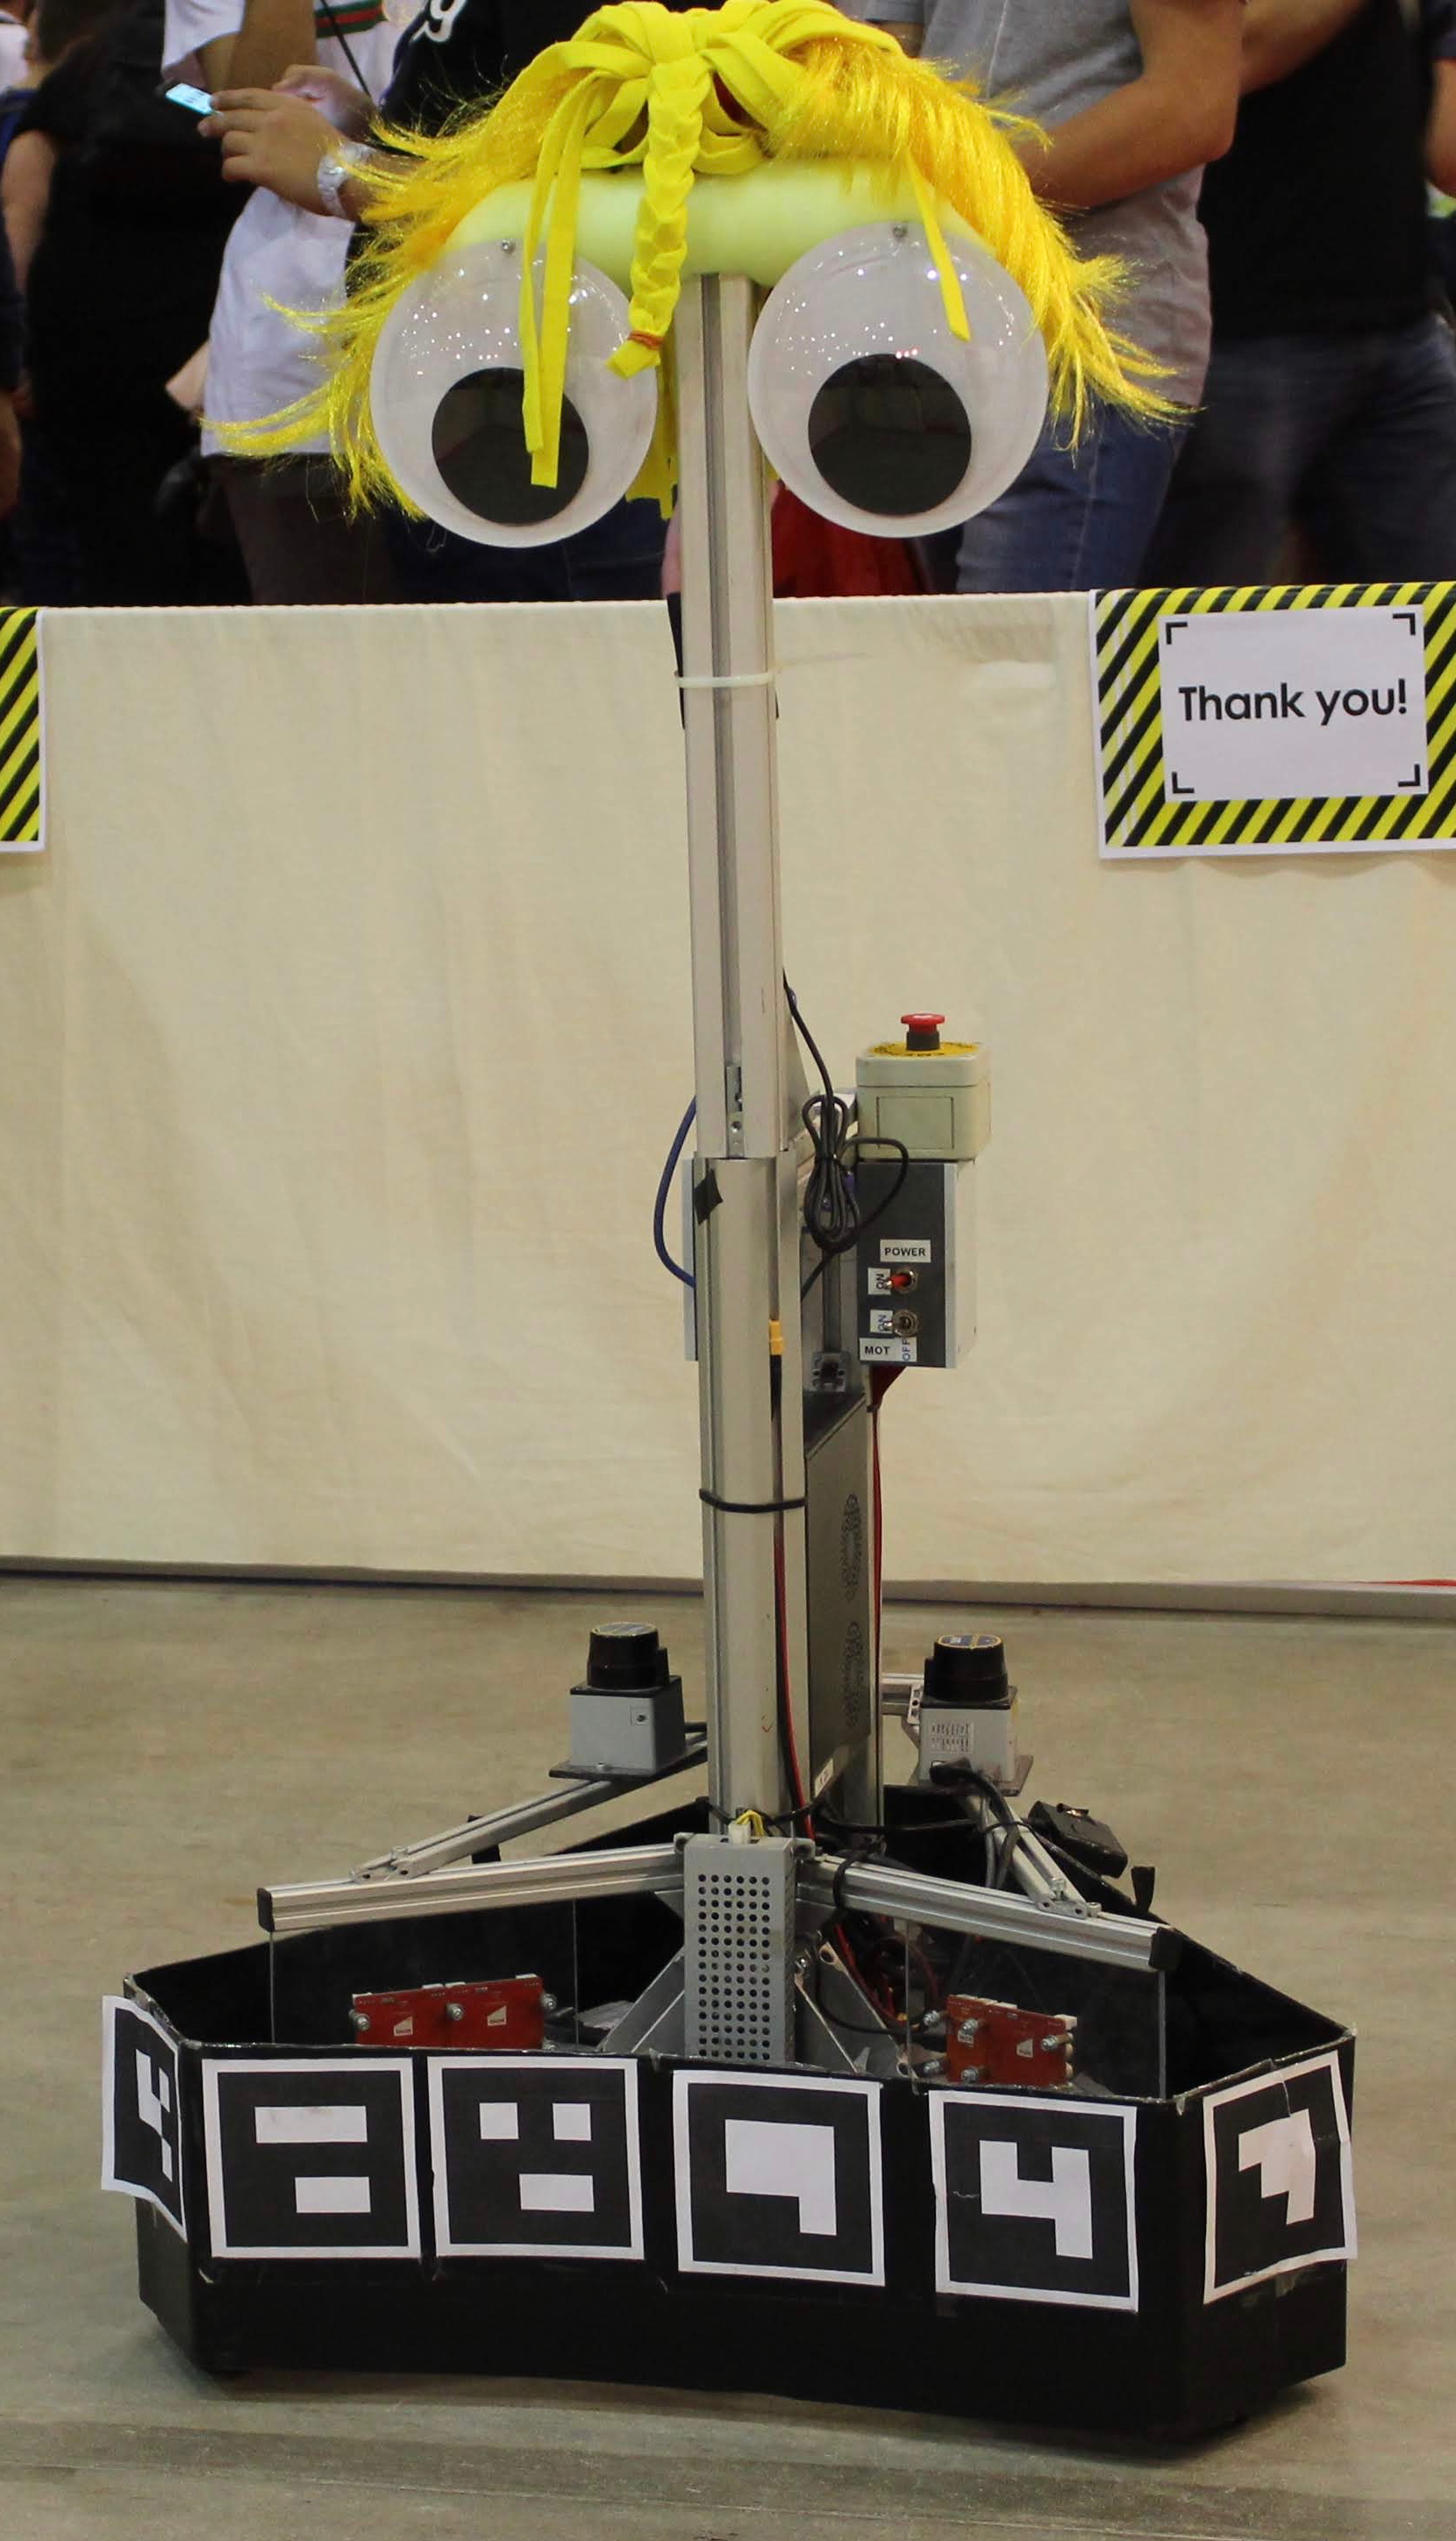
\includegraphics[width=3cm%,height=5.4cm
	      ]{images/03-foundation/base4.png}}}\label{newrobot}
	      \caption{}
      \end{subfigure}
      \caption{Prototype evolution. a) first version; b) second version differing on a button placed above the kinect; c) third version improving instability. d) fourth version including lasers on the base; e) current version during the Maker Faire 2018 in Rome (the European edition) from October 12th to 14th of 2018. A better placement of lasers has made the use of Kinect unnecessary.}
      \label{fig:evolution}
\end{figure}

\subsection{Sensors}
\subsubsection{Microsoft Kinect\textsuperscript{\textregistered}\label{sec:kinectsec}}
The Microsoft Kinect\textsuperscript{\textregistered} sensor is a 3-D camera: in addition to providing an RGB image with its 1080p color camera, it also provides a depth map,  meaning that for every pixel of the depth image provided by the sensor, Kinect\textsuperscript{\textregistered} provides the distance from the sensor. This makes the sensor suitable for a variety of computer vision problems like background removal, blob detection, and people tracking.

\begin{figure}[H]
	\centering
	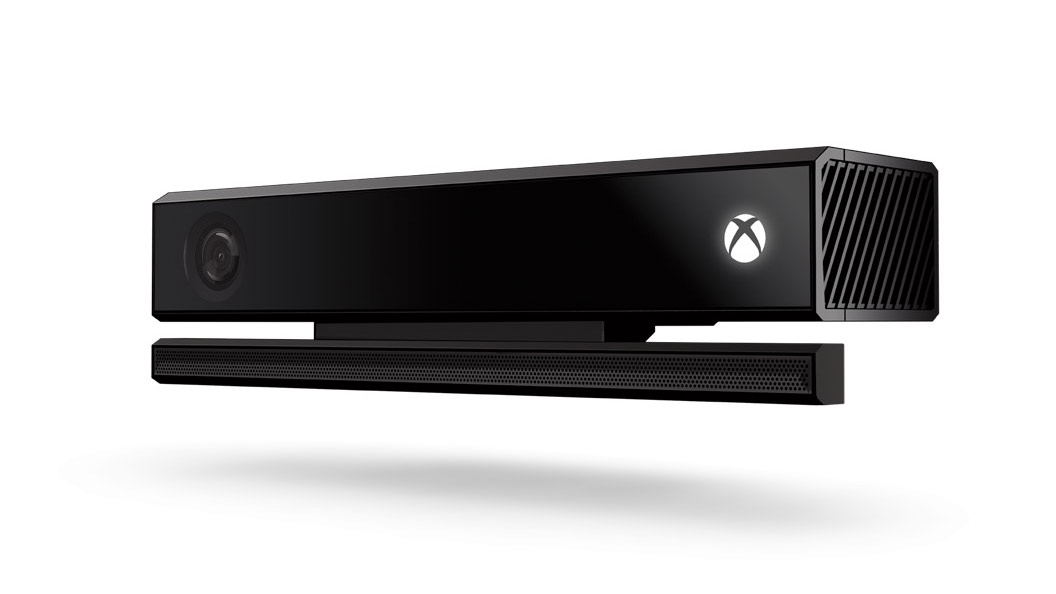
\includegraphics[width=5cm]{images/03-foundation/kinect}
	\caption{Kinect\textsuperscript{\textregistered} for Xbox ONE.}
	\label{kinect} 
\end{figure}

\begin{table}[H]
\begin{center}
	\begin{tabular}{|c|c|}
		\hline
		sensor dimensions & 24.9 cm $\times$ 6.6 cm $\times$ 6.7 cm\\
		\hline
		sensor weight & approximately 3.1 lbs (1.4 kg) \\
		\hline
		sensor FOV & 70\textsuperscript{$\circ$} x 60\textsuperscript{$\circ$} \\
		\hline
		depth sensing resolution & 512 x 424 \\
		\hline
		max - min depth & 4.5m - 0.4m \\ 
		\hline
		working frequency & 30 hz \\
		\hline 
	\end{tabular}
\end{center}
\caption{Kinect\textsuperscript{\textregistered} sensor features.}
\label{kinectfeatures}
\end{table}

We have used~\href{https://github.com/OpenKinect/libfreenect2}{libfreenect2}, a library for managing the Kinect\textsuperscript{\textregistered} device on Linux. We have then created a custom tracking node capable of estimating the player's position in two phases: First, color blob detection. Second, segmentation on the depth frame using~\href{https://en.wikipedia.org/wiki/Region_growing}{\textit{region growing}} algorithm for the purpose of detecting the player's body. Two features can be detected from this procedure: distance (relative to the robot) and contraction index. The first is calculated from the mean value of the depth pixels around the center of the blob. The latter is computed based on the subtraction of the occupied area with respect to the dimension of the bounding box that encompasses the segmented silhouette (see Figure~\ref{fig:segmenta}). This feature had been considered as a cue about the fact that the player was opening arms, so, possibly, actively participate to the game..

\begin{figure}[H]
  \centering 
  \begin{subfigure}[b]{0.3\textwidth}
		\centering
		\framebox{\parbox{3cm}{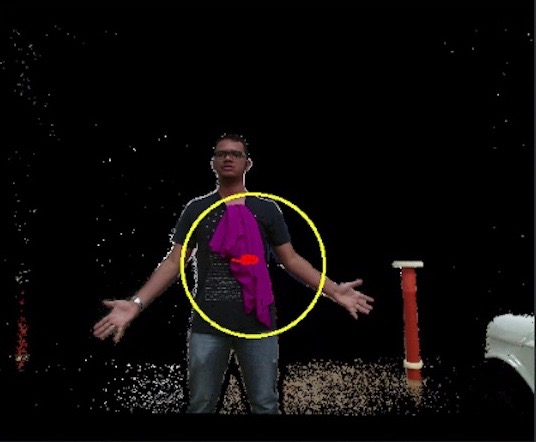
\includegraphics[width=3cm, height=3cm]{images/03-foundation/point_cloud}}}
		\caption{}
  \end{subfigure}
  ~
  \begin{subfigure}[b]{0.3\textwidth}
		\centering
		\framebox{\parbox{3cm}{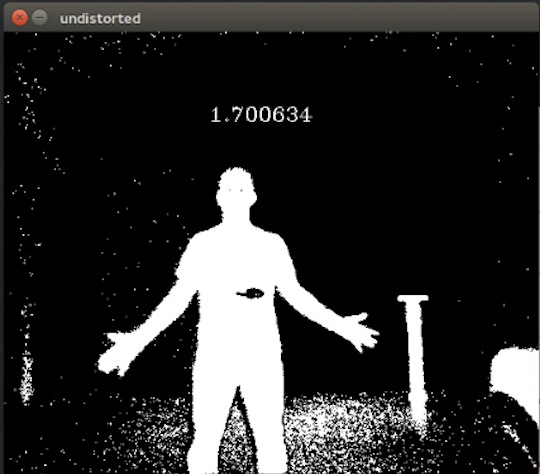
\includegraphics[width=3cm, height=3cm]{images/03-foundation/depth}}}
		\caption{}
  \end{subfigure}
  ~
  \begin{subfigure}[b]{0.3\textwidth}
		\centering
		\framebox{\parbox{3cm}{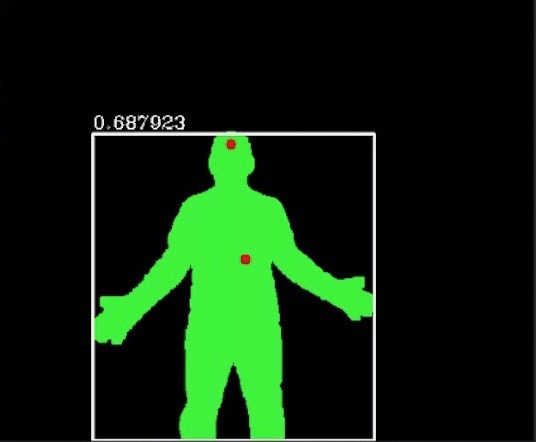
\includegraphics[width=3cm, height=3cm]{images/03-foundation/segmentation}}}
		\caption{}
  \end{subfigure}
  \caption{Example of Frames processed by our algorithm. a) Point cloud showing the center of the detected (light-purple) color blob. b) Depth frame. The number showed above the user correspond to his estimated distance relative to the robot. c) Segmentation results. The number above is the contraction index defined in the interval [0,1].}\label{fig:segmenta}
   \label{segmentacao}
\end{figure}

\subsubsection{Laser scanners}\label{lasershokuyo}
The robot was equipped with two laser scanners Hokuyo URG-04LX, shown in Figure~\ref{fig:hokuyo}. These laser sensors perceive the range of obstacles on a plan with a field of view of $240^\circ$ and a resolution of $0.36^\circ$, the maximum detectable distance is $5.6m$ and they can be connected to the computer by means of a USB interface, being operated with a nominal voltage of 5V.

The Hokuyo URG-04LX consists of a compact stacked structure with a spindle motor and the actual scanner on top of it. The motor rotates a small transmission mirror that deflects the vertical laser beam coming from the top of the sensor into horizontal direction. This allows the laser beam to scan a planar area around the sensor with an opening angle of $240^\circ$. A second mirror below, the reception mirror, deviates the horizontal laser beam captured by a lens into vertical direction again.

\begin{figure}[H]
	\centering
	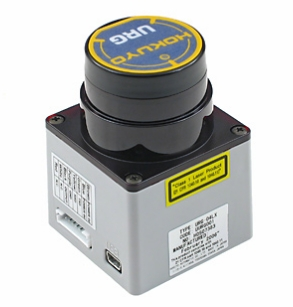
\includegraphics[width=5cm]{images/03-foundation/hokuyo}
	\caption{ An Hokuyo URG-04LX laser scanner.}
	\label{fig:hokuyo} 
\end{figure}

A full scan is performed every 100 ms. We mounted a laser scanner on each side of the lower chassis allowing for a $360^\circ$ coverage around the robot at a height of 30 cm from the floor.

\subsection{Motors}
The three motors are MAXON 118798 DC motor RE36 GB 70W KL 2WE, whose characteristics are reported in Figure~\ref{motor} and Table~\ref{maxon}.

\begin{figure}[H]
	\centering
	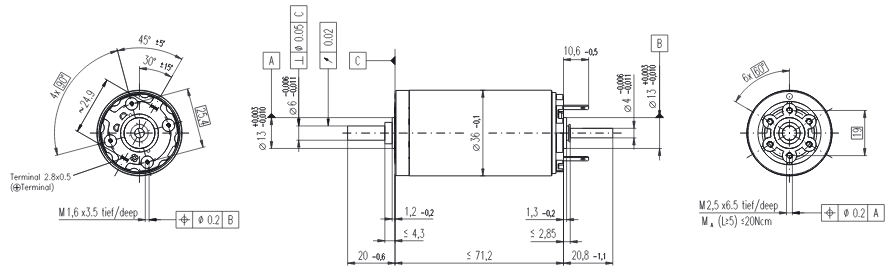
\includegraphics[width=\textwidth]{images/03-foundation/motor}
	\caption{Robot motors (3 units)}
	\label{motor} 
\end{figure}

\begin{table}[h]
	\begin{center}
		\begin{tabular}{|c|c|}
			\hline
			Assigned power rating &  70 W \\
			\hline
			Nominal voltage & 24 V \\
			\hline
			No load speed & 70 x 60  \\
			\hline
			Stall torque & 783 mNm \\
			\hline
			No load current & 105 mA \\ 
			\hline
			Terminal resistance & 1.11 ohm \\
			\hline 
			Max. permissible speed & 8200 rpm \\
			\hline
			Max. efficiency &  85\% \\
			\hline
			Torque constant & 36.4 mNm/A \\
			\hline
			Speed constant & 263 rpm/V \\
			\hline
			Mechanical time constant & 6 ms \\
			\hline 
			Rotor inertia & 67.7 gcm$^2$ \\
			\hline
			Terminal Inductance & 0.2 mH \\
			\hline  
			reduction ratio & [14 : 1] (166158 planetary gear GP32A 2.25NM) \\
			\hline 
		\end{tabular}
	\end{center}
	\caption{MAXON 118798 DC motor parameters.}
    \label{maxon}
\end{table}

\subsubsection{Encoders}
On each motor a 110513 tacho ENCODER HEDS 5540 500IMP 3K is mounted to get the speed of the motor, whose characteristics are reported in Figure~\ref{enc}.
\begin{figure}[htbp]
	\centering
	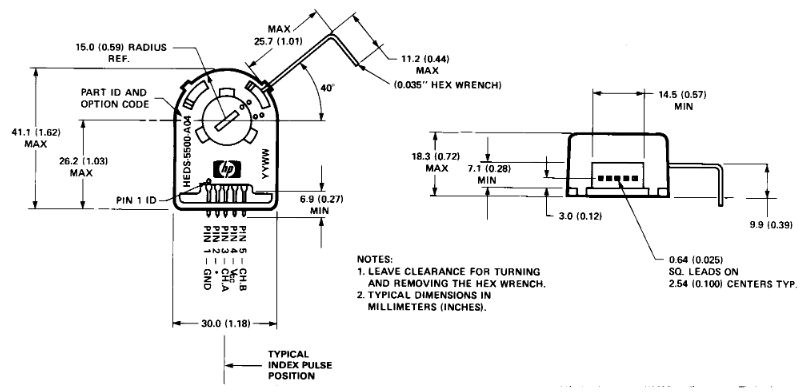
\includegraphics[width=\textwidth]{images/03-foundation/enc}
	\caption{Motor encoders deployed for motion sensing and control.}
	\label{enc} 
\end{figure}
Encoders contain a single Light Emitting Diode (LED) as its light source. The light is collimated into a parallel beam by means of a single lens located directly over the LED. Opposite the emitter is the integrated detector circuit. This IC consists of multiple sets of photodetectors and the signal processing circuitry necessary to produce the digital waveforms. The code-wheel rotates between the emitter and detector, causing the light beam to be interrupted by the pattern of spaces and bars on the code-wheel. The photodiodes detect these interruptions and send signals to the signal processing circuitry that produces the final outputs that is an index pulse $P_O$ which is generated once for each full rotation of the code-wheel.

\subsection{Onboard computer}
\label{onboard pc}
For computing a Shuttle XPC Slim DH270 was used. The device has a $190 \times 165 \times 43$~mm steel case, and weights $1.3$~kg.  The armature presents two holes for Kensington Locks and numerous threaded holes (M3) at both sides allowing for an easy placement. The operating system used was the~\textit{Ubuntu 16.04.3 LTS (64bit)}.

\begin{figure}[H]
	\centering
	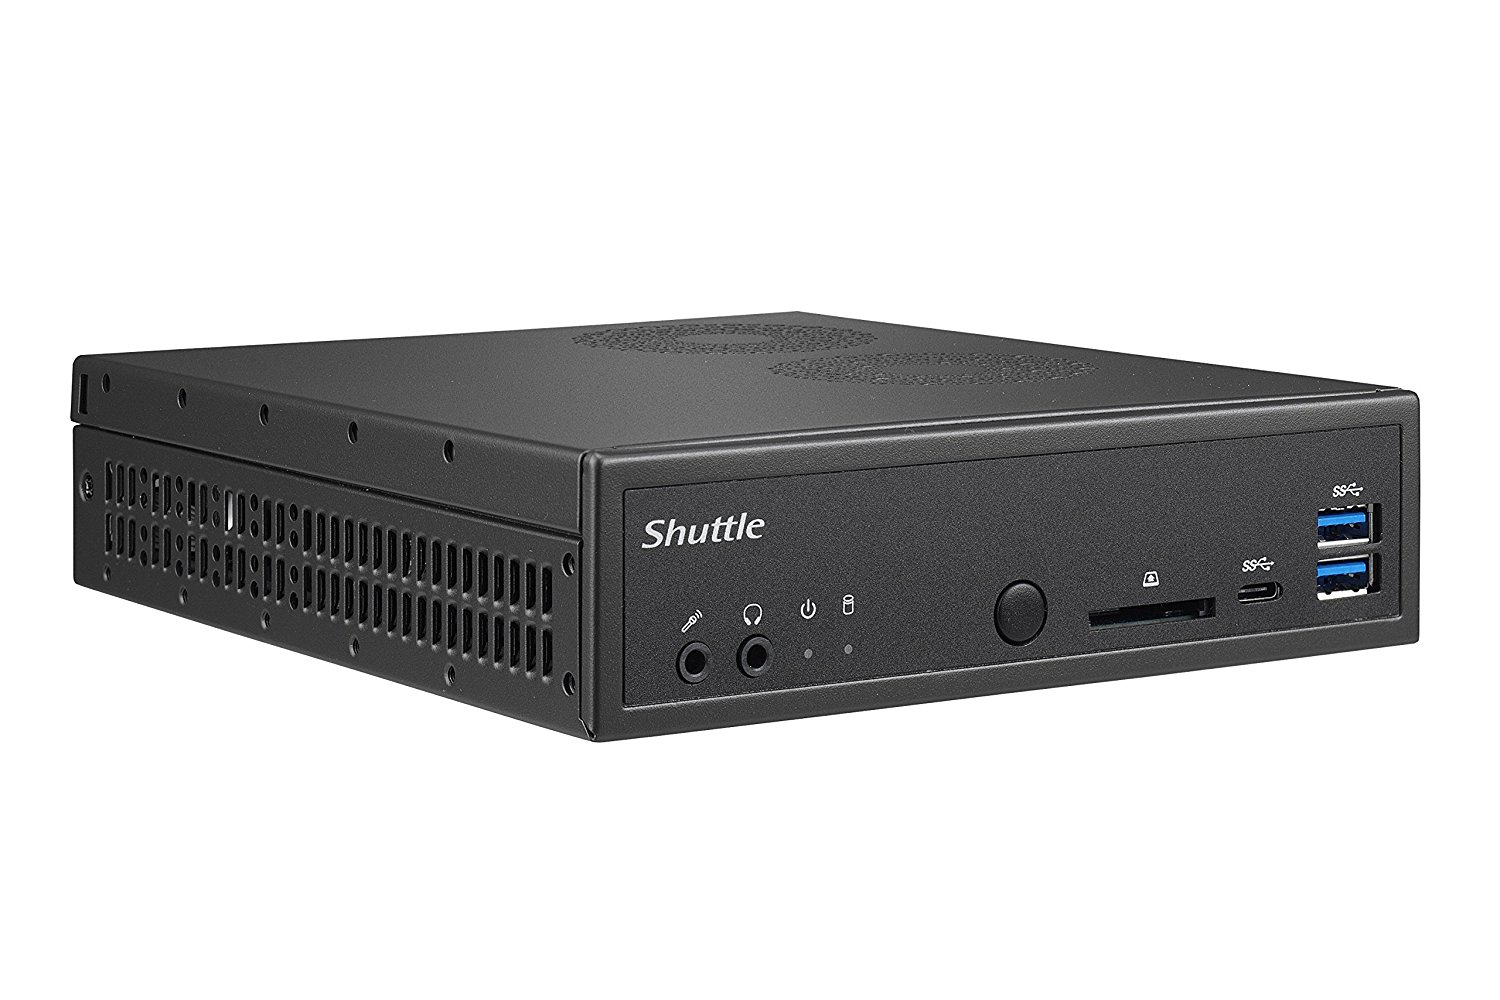
\includegraphics[width=6cm]{images/03-foundation/onboardpc}
	\caption{The on-board pc, Shuttle XPC Slim DH270: barebone Intel Kaby-Lake. Processor Intel Core i7; RAM memory of 16 GB DDR4.}
	\label{onboardpc}
\end{figure}

\subsection{The control boards}
\label{novacore}
The low-level motors actuation and their interface between the ROS system have been realized with the Nova Core modules based on STM32-chip~\cite{noauthor_nova_nodate}, which implement ready to use components to fulfill robot prototyping requirements with plug \& play approach.  
The provided modules allow to control different type of motors that can be modeled as a second order system, where the input is the voltage applied to the motor armature and output variable is the motor angular speed. Futher details about the deployed boards are presented in figure~\ref{fig:boards}.


\begin{figure}[H]
  \centering
  \begin{subfigure}[b]{0.3\textwidth}
  \centering
      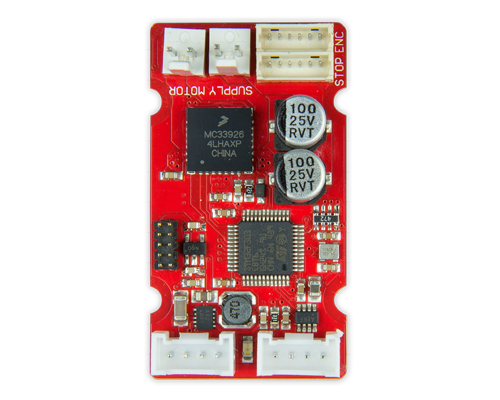
\includegraphics[width=3cm,height=3cm]{images/03-foundation/udc}
	\caption{}
  \end{subfigure}
  \begin{subfigure}[b]{0.3\textwidth}
  \centering
      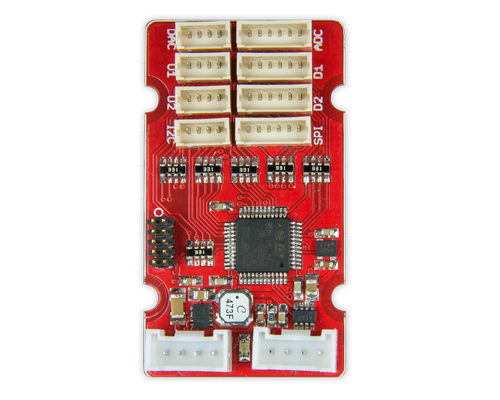
\includegraphics[width=3cm,height=3cm]{images/03-foundation/io}
	\caption{}
  \end{subfigure}
  \begin{subfigure}[b]{0.3\textwidth}
  \centering
      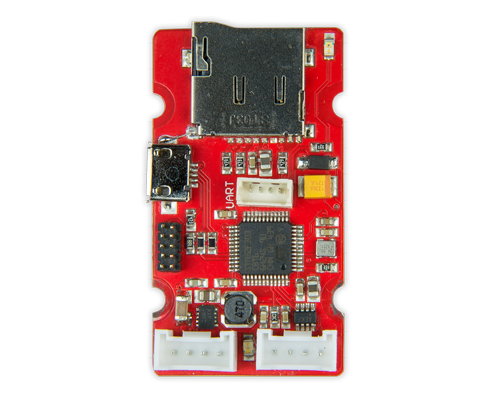
\includegraphics[width=3cm,height=3cm]{images/03-foundation/usb}
	\caption{}
	\label{fig:usb_board}
  \end{subfigure}
  \caption{a) UDC board (1 per each motor) capable of driving motors up to 70 W, with torque, speed, and position closed loop control. General attributes: 5-28V supply; 3A max (5A peak); current sense; encoder input; limit switch input; 25 x 45 mm in size. b) IO board (1 per each motor): Integrate existing hardware into the real-time Nova Core bus with analog and digital signals. General attributes: 8 digital GPIO;  4 analog inputs; 2 analog outputs; 2 UART; 1 I2C; 1 SPI; 25 x 45 mm in size. c) USB board (used for data collection) Interface the real-time Nova Core bus with a computer and logs data to microSD memory. General attributes: USB connector;  UART connector; microSD card slot; rosserial support; 25 x 45 mm in size.}
  \label{fig:boards}
\end{figure}
%ANDY all the technical details and names of devices could go in an appendix, while I'll leave here a functional description of robot and sensors, giving the characteristics that are functionally relevant, e.g., speed, omnidirectionality, range of sensors, their data rate, ...

\subsection{Kinematics}\label{sec:kinematics}

%ANDY This is a definition that could be given for granted -> Kinematics is a branch of classical mechanics that describes the motion of points, bodies, and systems of bodies without considering the mass of each or the forces that caused the motion.


%ANDY Actually, all this section can be an appendx. It is not entral to your thesis.

The pose of a rigid mobile robot is commonly described by six variables, its three-dimensional Cartesian coordinates and its three Euler angles (roll, pitch, yaw) relative to an external coordinate frame~\cite{thrun_probabilistic_2005}. If the robot is considered as moving on a planar surface, this reduces to two Cartesian coordinates and an orientation angle.
The kinematic model of an omni-directional base consists of an equation of motion of the robot in function of wheels velocity without considering the forces acting on the system. In this section, a kinematic model for a 3-wheeled omni-directional robot will be derived.

\begin{figure}[H]
  \centering
  \begin{subfigure}[b]{0.5\textwidth}
     \centering
      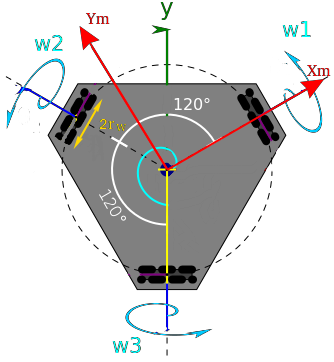
\includegraphics[width=5cm]{images/03-foundation/triskarbase1}
	\caption{}
	\label{triskar1} 
  \end{subfigure}
  \begin{subfigure}[b]{0.5\textwidth}
  \centering
      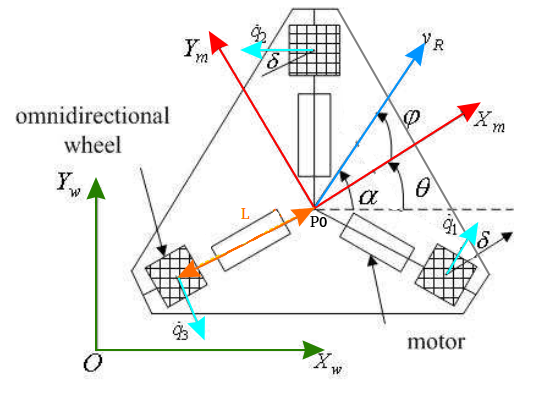
\includegraphics[width=5cm]{images/03-foundation/triskarbase2}
	\caption{}
	\label{triskar2} 
  \end{subfigure}
  \caption{Kinematics diagram of the base of an omnidirectional robot. a) omni-directional base wheels displacement angle. b) omni-directional base reference frames and velocities.}
\end{figure}

Considering the figure (\ref{triskar2}), each wheel of the robot is driven by a DC motor and its center has the same distance L to the robot center of mass $P_0$. we define the fixed world coordinate system [$X_R$, $Y_R$] and a mobile robot fixed frame [${x}^m_R$, ${y}^m_R$] that is parallel to the floor and whose origin locates at $P_0$.\\
The robot's orientation is denoted by angle $\theta$, which is the direction angle of the axis $X_m$ in the world coordinate system (positive in the
counterclockwise direction) and $\delta$ refers to the wheel orientation in the robot coordinate system and it is equal to 30 degrees in our considered example.
\\
$\alpha$ and $\phi$ denote the direction of the robot translation velocity $v_R$ observed in the world and robot coordinate systems, respectively.\\
We consider \textbf{v} = [$\dot{x}^m_R,\dot{y}^m_R,\omega$]$^T$ the robot velocities observed in the robot coordinate system; \\
$\mathbf{\dot{q}}$ = [$\dot{q}_1,\dot{q}_2,\dot{q}_3$]$^T$ is the vector of wheel velocities equal to the i-th wheel radius $r_\omega$ multiplied by the wheel angular velocity.

We introduce the transformation matrix from the robot coordinate system to the world coordinate system:
\begin{equation}
^wR_m(\theta)=\begin{bmatrix}
\cos(\theta) &-\sin(\theta)\\
\sin(\theta) & \cos(\theta)\\
\end{bmatrix}
\end{equation}

We can transform from robot to world coordinates system as:
\begin{equation}
\begin{bmatrix}
\dot{x}_R\\
\dot{y}_R\\
\dot{\theta}
\end{bmatrix} =
\begin{bmatrix}
\cos(\theta) &-\sin(\theta) & 0\\
\sin(\theta) & \cos(\theta) & 0\\
0 & 0 & 1
\end{bmatrix}
\begin{bmatrix}
\dot{x}^m_R\\
\dot{y}^m_R\\
\omega
\end{bmatrix}
\label{rotation}
\end{equation}

$P_0$ denotes the position of the center of mass with respect to the world frame as:
\begin{equation}
P_0 = 	\begin{bmatrix}
x_R\\
y_R\\
\end{bmatrix}
\end{equation}

The position $[x_i\quad y_i]^T$ of each wheel can be given with respect to the center of mass of the robot, for i=1,2,3:
\begin{equation}
P_i = 	\begin{bmatrix}
x_{Ri}\\
y_{Ri}\\
\end{bmatrix} = 
^wR_m(\theta)\cdot L
\begin{bmatrix}
1\\
0\\
\end{bmatrix}
\end{equation}

Again, considering that the wheels present a displacement of $120^\circ$ between each other we can deduce the following three vectors:

\begin{equation}
\begin{cases} 
P_1 = 	
^wR_m(0)\cdot L
\begin{bmatrix}
1\\
0\\
\end{bmatrix} =
L
\begin{bmatrix}
1\\
0\\
\end{bmatrix}
\\ 
P_2 = 	
^wR_m(\frac{2\pi}{3})\cdot L
\begin{bmatrix}
1\\
0\\
\end{bmatrix} =
\cfrac{L}{2}
\begin{bmatrix}
-1\\
\sqrt{3}\\
\end{bmatrix}
\\ 
P_3 = 	
^wR_m(\frac{4\pi}{3})\cdot L
\begin{bmatrix}
1\\
0\\
\end{bmatrix} =
-\cfrac{L}{2}
\begin{bmatrix}
-1\\
\sqrt{3}\\
\end{bmatrix}
\\ 
\end{cases} 
\end{equation}

We now define the normal unit vectors of each wheel, representing the translational direction, as follows:
\begin{equation}
D_i =  \frac{1}{L}R(\frac{\pi}{2})P_i\qquad i=1,2,3 \\
\end{equation}
\begin{equation}
\begin{cases}
D_1 = \begin{bmatrix}0 \\ 1 \end{bmatrix} \\
D_2 = -\cfrac{1}{2}\begin{bmatrix}\sqrt{3} \\ 1 \end{bmatrix} \\
D_3 = \cfrac{1}{2}\begin{bmatrix}\sqrt{3} \\ -1 \end{bmatrix} \\
\end{cases}
\end{equation}

Then the translational velocity $q_i$ as depicted in figure~\ref{triskar2} can be written in the robot reference frame as follows:
\begin{equation}
\begin{cases}
\dot{q_1} =\cos(\delta)\dot{x^m _R}+\sin(\delta)\dot{y^m _R}+L{\omega}\\
\dot{q_2} =-\cos(\delta)\dot{x^m _R}+\sin(\delta)\dot{y^m _R}+L{\omega}\\
\dot{q_3} =-\dot{y^m _R}+L{\omega}\\
\end{cases}
\end{equation}

The kinematic model with respect to the robot coordinate system is given by:
\begin{equation}
\begin{bmatrix}
\dot{x}^m _R\\
\dot{y}^m _R\\
{\omega}
\end{bmatrix} =
\begin{bmatrix}
\cos(\delta) & \sin(\delta) & L\\
-\cos(\delta) & \sin(\delta) & L\\
0 & -1 & L
\end{bmatrix}^{-1}
\begin{bmatrix}
\dot{q_1}\\
\dot{q_2}\\
\dot{q_3}\\
\end{bmatrix}	
\label{model1}
\end{equation}
\begin{equation*}
	\begin{bmatrix}
		\dot{x}^m _R\\
		\dot{y}^m _R\\
		{\omega}
	\end{bmatrix} =
	\begin{bmatrix}
		\frac{\sqrt{3}}{3} & -\frac{\sqrt{3}}{3} & 0\\
		\frac{1}{3} & \frac{1}{3} & -\frac{2}{3}\\
		\frac{1}{3L} & \frac{1}{3L} & \frac{1}{3L}
	\end{bmatrix}
	\begin{bmatrix}
		\dot{q_1}\\
		\dot{q_2}\\
		\dot{q_3}\\
	\end{bmatrix}	
\end{equation*}

If we now consider the equation~\ref{rotation} the kinematic model with respect to the world coordinate system is described as:
\begin{equation}
\begin{bmatrix}
\dot{x}_R\\
\dot{y}_R\\
\dot{\theta}
\end{bmatrix} =
\begin{bmatrix}
\frac{2}{3}\cos(\theta+\delta) & -\frac{2}{3}\cos(\theta-\delta) & \frac{2}{3}\sin(\theta)\\
\frac{2}{3}\sin(\theta+\delta) & -\frac{2}{3}\sin(\theta-\delta) & \frac{2}{3}\cos(\theta)\\
\frac{1}{3L} & \frac{1}{3L} & \frac{1}{3L}
\end{bmatrix}
\begin{bmatrix}
\dot{q_1}\\
\dot{q_2}\\
\dot{q_3}\\
\end{bmatrix}	
\label{model2}
\end{equation}

where $\mathbf{\dot{x}}$ = [$\dot{x}_R,\dot{y}_R,\dot{\theta}$]$^T$ is the robot velocity vector with respect to the world coordinate system;

It is important to notice that the transformation matrix in model~\ref{model1} is full rank, which denotes that the translation and rotation of the robot are decoupled, and guarantees the separate control of these two movements.

Low level actuation (such as velocity control of the wheels) is embedded in the robot boards and, after considering figure~\ref{triskar1} and figure~\ref{triskar2}, we can define a system of equations that describes the angular velocity of each wheel.\\	
If we define $[\omega R_1; \omega R_2; \omega R_3]^T$ as the wheel angular velocities vector, we have:
\begin{equation}
\begin{cases} 

\omega_{R1} = \dot{x}^m_R\cos(\delta)+\dot{y}^m_R\sin(\delta)+ \omega L\\ 
\omega_{R2} = -\dot{x}^m_R\cos(\delta)+\dot{y}^m_R\sin(\delta)+\omega L\\ 
\omega_{R3} = -\dot{y}^m_R +  \omega L \\ 
\end{cases} 
\end{equation}
This can be written in matrix form as:
\begin{equation}
\begin{bmatrix}
\omega_{R1}\\
\omega_{R2}\\
\omega_{R3}
\end{bmatrix} = 
\begin{bmatrix}
\cos(\delta) & \sin(\delta) & L \\
-\cos(\delta) & \sin(\delta) & L \\
0 & -1 & L
\end{bmatrix}
\begin{bmatrix}
\dot{x}^m_R\\
\dot{y}^m_R\\
\omega
\end{bmatrix}
\end{equation} 
As previously anticipated we can also say:
\begin{equation}
\begin{bmatrix}
\dot{q_1}\\
\dot{q_2}\\
\dot{q_3}\\
\end{bmatrix} = 
r_\omega
\begin{bmatrix}
\omega_{R1}\\
\omega_{R2}\\
\omega_{R3}
\end{bmatrix}
\end{equation}
It is also known that a further relation between motor velocity and wheel velocity exists and is given by the equation:
\begin{equation}
\omega_{Ri}=\frac{r_\omega}{\eta N}\omega_{mi}
\end{equation}
for i=1,2,3 where $r_\omega$ is the wheel radius, N is the coupling factor and $\eta$ is the wheel/motor coupling efficiency factor.

The direct kinematic for an holonomic robot can be finally written as:
\begin{equation}
\begin{bmatrix}
\dot{x}_R\\
\dot{y}_R\\
\dot{\theta}
\end{bmatrix} =
\begin{bmatrix}
\frac{2}{3}\cos(\theta+\delta) & -\frac{2}{3}\cos(\theta-\delta) & \frac{2}{3}\sin(\theta)\\
\frac{2}{3}\sin(\theta+\delta) & -\frac{2}{3}\sin(\theta-\delta) & \frac{2}{3}\cos(\theta)\\
\frac{1}{3L} & \frac{1}{3L} & \frac{1}{3L}
\end{bmatrix}
\frac{r_\omega}{\eta N}
\begin{bmatrix}
\omega_{m1}\\
\omega_{m2}\\
\omega_{m3}
\end{bmatrix}
\label{directkin}
\end{equation}
\paragraph{Inverse Kinematic:} If we reverse and re-arrange equation~\ref{directkin} we obtain:
\begin{equation}
B = \begin{bmatrix}
\frac{2}{3}\cos(\theta+\delta) & -\frac{2}{3}\cos(\theta-\delta) & \frac{2}{3}\sin(\theta)\\
\frac{2}{3}\sin(\theta+\delta) & -\frac{2}{3}\sin(\theta-\delta) & \frac{2}{3}\cos(\theta)\\
\frac{1}{3L} & \frac{1}{3L} & \frac{1}{3L}
\end{bmatrix}
\end{equation}
\begin{equation}
\begin{bmatrix}
\dot{x}_R\\
\dot{y}_R\\
\dot{\theta}
\end{bmatrix} =
B
\frac{r_\omega}{\eta N}
\begin{bmatrix}
\omega_{m1}\\
\omega_{m2}\\
\omega_{m3}
\end{bmatrix}
\end{equation}
\begin{equation}
\begin{bmatrix}
\omega_{m1}\\
\omega_{m2}\\
\omega_{m3}
\end{bmatrix}=
\frac{\eta N}{r_\omega}B^{-1}
\begin{bmatrix}
\dot{x}_R\\
\dot{y}_R\\
\dot{\theta}
\end{bmatrix}
\label{inversekin}
\end{equation}
Equation~\ref{inversekin} represents the inverse kinematic model for the considered holonomic robot that bounds the robot velocities in the inertial reference frame to the actual motors velocities.
